\section{Pr\'esentation du sujet}

\subsection{Le projet Yuukou}

\begin{frame}{Le projet \textit{Yuukou}}
	\begin{figure}[h]
		\centering
		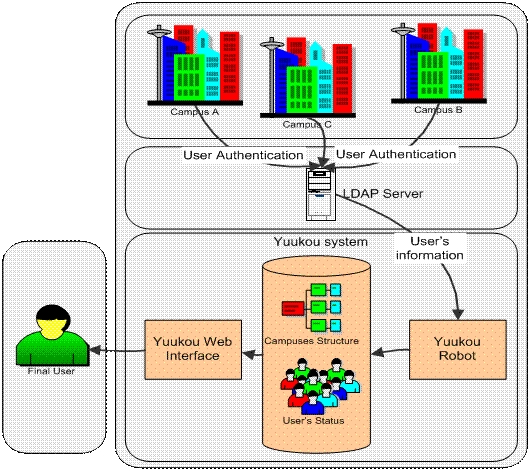
\includegraphics[scale=0.435]{yuukouFonctionnement.jpg}
	
	\end{figure}
	
\end{frame}

%%%%%%%%%%%%%%%%%%%%%%%%%%%%%%%%%

\begin{frame}{Le projet \textit{Yuukou}}
	\begin{block}{Fonctionnalit\'es de \textit{Yuukou}}
		\begin{itemize}
			\item Collecte et affichage des donn\'ees LDAP
			\item Disponibilit\'e des salles informatiques
			\item Pages publiques et priv\'ees
			
		\end{itemize}
		
	\end{block}
	
	\begin{block}{Pages publiques}
		\begin{itemize}
			\item Utilisateur normal (\'etudiant)
			\item Vision g\'en\'erale des salles informatiques
			
		\end{itemize}
		
	\end{block}
	
	\begin{block}{Pages priv\'ees}
		\begin{itemize}
			\item Administrateur
			\item Identification avec LDAP
			\item Reprise des pages publiques avec plus de d\'etails
			
		\end{itemize}
		
	\end{block}
	
\end{frame}

%%%%%%%%%%%%%%%%%%%%%%%%%%%%%%%%%

\begin{frame}{Le projet \textit{Yuukou}}
	\begin{block}{D'un point de vue technique}
		\begin{itemize}
			\item D\'evelopp\'e avec Perl pour le robot
			\item Pages Web en PHP
			\item Stockage des informations dans MySQL
			\item Utilisation de eDirectory de Novell
			
		\end{itemize}
		
	\end{block}
	
	\begin{block}{Quelques chiffres}
		\begin{itemize}
			\item 43 salles informatiques
			\item 661 PC
			\item Pas de Macintosh
			
		\end{itemize}
		
	\end{block}
	
\end{frame}

%%%%%%%%%%%%%%%%%%%%%%%%%%%%%%%%%

\begin{frame}{Le projet \textit{Yuukou}}
	\begin{figure}[h]
		\centering
		\only<1>{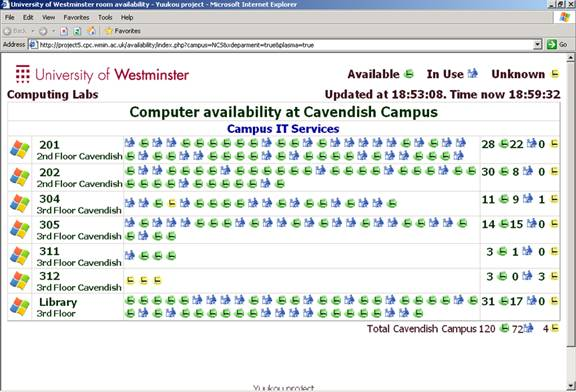
\includegraphics[scale=0.625]{yuukouPublic.jpg}}
		\only<2>{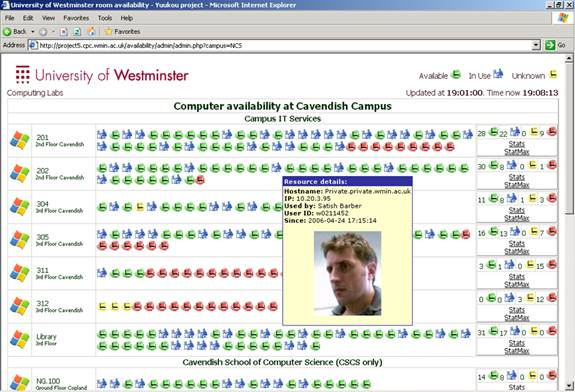
\includegraphics[scale=0.625]{yuukouAdmin.jpg}}
			
	\end{figure}
	
\end{frame}

%%%%%%%%%%%%%%%%%%%%%%%%%%%%%%%%%

\begin{frame}{Le projet \textit{Yuukou}}
	\begin{block}{Changement vers \textit{Yuukou II}}
		\begin{itemize}
			\item Personne pour maintenir ou \'etendre \textit{Yuukou}
			\item Changement vers Active Directory de Windows
			\item Pas de Macintosh
			\item Pas d'historique
			\item Pas d'emploi du temps donc faussement des r\'esultats
			\item Simplifier l'acc\`es aux \'etudiants
			
		\end{itemize}
		
	\end{block}
	
\end{frame}

%%%%%%%%%%%%%%%%%%%%%%%%%%%%%%%%%

\subsection{Le projet Yuukou II}

\begin{frame}{Pr\'esentation du sujet}
	\begin{block}{Le sujet}
		\begin{itemize}
			\item Combler les lacunes de \textit{Yuukou}
			\item Aller plus loin en termes de fonctionnalit\'es
			\item But : cr\'eation d'un service Web
			\item Finalit\'e : fournir un projet pilote pour les \'equipes de l'Universit\'e
			
		\end{itemize}
		
	\end{block}
	
	\begin{block}{D\'ecoupage du sujet}
		\begin{itemize}
			\item Partie service Web
			\item Partie affichage : M. Yacine MAGHEZZI
			
		\end{itemize}
		
	\end{block}
	
\end{frame}

%%%%%%%%%%%%%%%%%%%%%%%%%%%%%%%%%

\subsection{Les objectifs principaux}

\begin{frame}{Pr\'esentation du sujet}
	\begin{block}{Les objectifs principaux}
		\begin{itemize}
			\item Service Web
			\item R\'ecup\'eration des informations des ordinateurs avec Nagios
			\item Base de donn\'ees pour archivage
			\item Cycle principal
			\item Multiples fonctions pour un client
			\item Structures de retour des informations
			\item Emplois du temps
			
		\end{itemize}
		
	\end{block}
	
\end{frame}

%%%%%%%%%%%%%%%%%%%%%%%%%%%%%%%%%

\subsection{Les contraintes techniques}

\begin{frame}{Les contraintes techniques}
	\begin{block}{Outils g\'en\'eraux}
		\begin{itemize}
			\item Service Web : Java avec JAX-WS
			\item R\'ecup\'eration des donn\'ees : Nagios
			\item Logiciels libres si besoin
			\item Syst\`eme d'exploitation UNIX
			
		\end{itemize}
		
	\end{block}
	
\end{frame}
